\section{Packet Class Reference}
\label{classPacket}\index{Packet@{Packet}}
{\tt \#include $<$packet.h$>$}

Inheritance diagram for Packet::\begin{figure}[H]
\begin{center}
\leavevmode
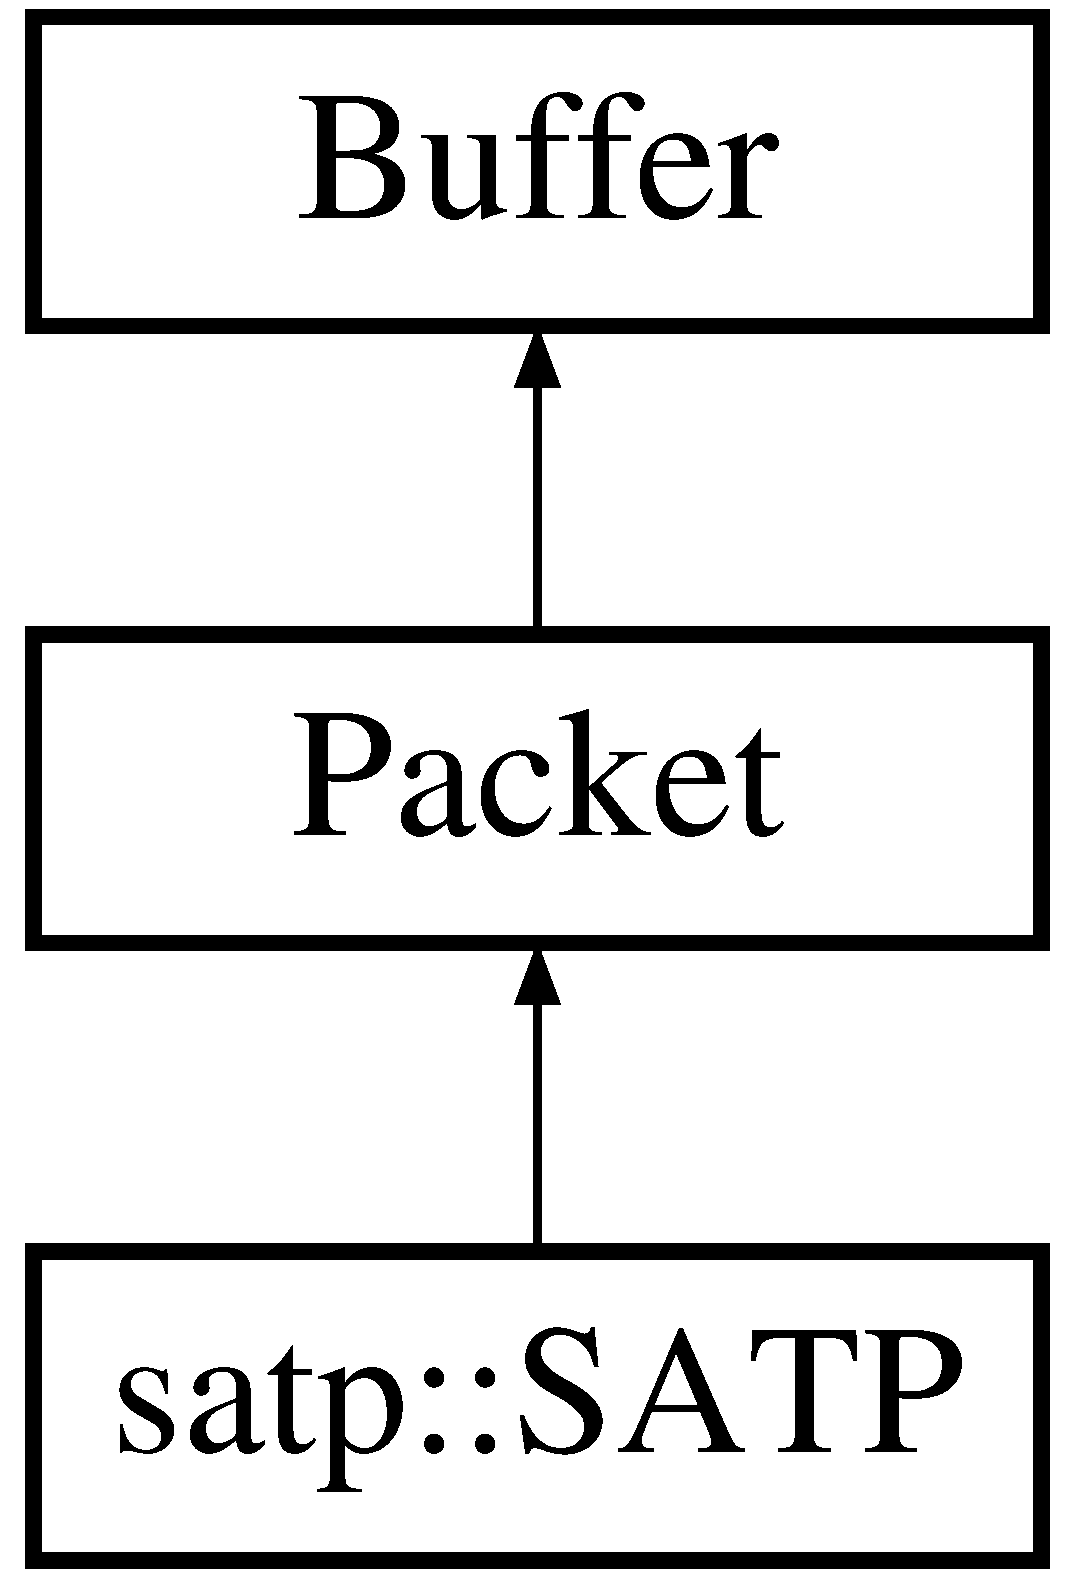
\includegraphics[height=3cm]{classPacket}
\end{center}
\end{figure}
\subsection*{Public Member Functions}
\begin{CompactItemize}
\item 
{\bf Packet} ()
\item 
{\bf Packet} ({\bf u\_\-int32\_\-t} length)
\item 
{\bf Packet} (const {\bf Buffer} \&src)
\item 
bool {\bf has\-Header} () const
\item 
{\bf Packet} \& {\bf with\-Header} (bool b)
\item 
{\bf seq\_\-nr\_\-t} {\bf get\-Seq\-Nr} () const
\item 
{\bf sender\_\-id\_\-t} {\bf get\-Sender\-Id} () const
\item 
{\bf Packet} \& {\bf add\-Header} ({\bf seq\_\-nr\_\-t} seq\_\-nr, {\bf sender\_\-id\_\-t} sender\_\-id)
\item 
{\bf Packet} \& {\bf remove\-Header} ()
\item 
{\bf Packet} \& {\bf set\-Seq\-Nr} ({\bf seq\_\-nr\_\-t} seq\_\-nr)
\item 
{\bf Packet} \& {\bf set\-Sender\-Id} ({\bf sender\_\-id\_\-t} sender\_\-id)
\item 
bool {\bf has\-Payload\-Type} () const
\item 
{\bf Packet} \& {\bf with\-Payload\-Type} (bool b)
\item 
{\bf payload\_\-type\_\-t} {\bf get\-Payload\-Type} () const
\item 
{\bf Packet} \& {\bf add\-Payload\-Type} ({\bf payload\_\-type\_\-t} payload\_\-type)
\item 
{\bf Packet} \& {\bf remove\-Payload\-Type} ()
\item 
bool {\bf has\-Auth\-Tag} () const
\item 
{\bf Packet} \& {\bf with\-Auth\-Tag} (bool b)
\item 
{\bf auth\_\-tag\_\-t} {\bf get\-Auth\-Tag} () const
\item 
{\bf Packet} \& {\bf add\-Auth\-Tag} ({\bf auth\_\-tag\_\-t} auth\_\-tag)
\item 
{\bf Packet} \& {\bf remove\-Auth\-Tag} ()
\end{CompactItemize}
\subsection*{Private Attributes}
\begin{CompactItemize}
\item 
{\bf Packet::Header\-Struct} {\bf \_\-\_\-packed\_\-\_\-}
\item 
bool {\bf has\_\-header\_\-}
\item 
bool {\bf has\_\-payload\_\-type\_\-}
\item 
bool {\bf has\_\-auth\_\-tag\_\-}
\end{CompactItemize}
\subsection*{Classes}
\begin{CompactItemize}
\item 
struct {\bf Header\-Struct}
\end{CompactItemize}


\subsection{Constructor \& Destructor Documentation}
\index{Packet@{Packet}!Packet@{Packet}}
\index{Packet@{Packet}!Packet@{Packet}}
\subsubsection{\setlength{\rightskip}{0pt plus 5cm}Packet::Packet ()}\label{classPacket_abcfb963c0d5bc0fa554668f92989622}


\index{Packet@{Packet}!Packet@{Packet}}
\index{Packet@{Packet}!Packet@{Packet}}
\subsubsection{\setlength{\rightskip}{0pt plus 5cm}Packet::Packet ({\bf u\_\-int32\_\-t} {\em length})}\label{classPacket_d2a8f6ac3d6de9b541708c4b0c73d04b}


\index{Packet@{Packet}!Packet@{Packet}}
\index{Packet@{Packet}!Packet@{Packet}}
\subsubsection{\setlength{\rightskip}{0pt plus 5cm}Packet::Packet (const {\bf Buffer} \& {\em src})}\label{classPacket_27264b7d411a74ea9a0077bf5f9222b1}




\subsection{Member Function Documentation}
\index{Packet@{Packet}!hasHeader@{hasHeader}}
\index{hasHeader@{hasHeader}!Packet@{Packet}}
\subsubsection{\setlength{\rightskip}{0pt plus 5cm}bool Packet::has\-Header () const}\label{classPacket_a004c01dd99179b0a08109dce5fc6b03}


\index{Packet@{Packet}!withHeader@{withHeader}}
\index{withHeader@{withHeader}!Packet@{Packet}}
\subsubsection{\setlength{\rightskip}{0pt plus 5cm}{\bf Packet} \& Packet::with\-Header (bool {\em b})}\label{classPacket_ce9e40180f64d44fe1d8da14ac9e5df2}


\index{Packet@{Packet}!getSeqNr@{getSeqNr}}
\index{getSeqNr@{getSeqNr}!Packet@{Packet}}
\subsubsection{\setlength{\rightskip}{0pt plus 5cm}{\bf seq\_\-nr\_\-t} Packet::get\-Seq\-Nr () const}\label{classPacket_6572b9df8c1f5f0de9fcb8e5c669de50}


\index{Packet@{Packet}!getSenderId@{getSenderId}}
\index{getSenderId@{getSenderId}!Packet@{Packet}}
\subsubsection{\setlength{\rightskip}{0pt plus 5cm}{\bf sender\_\-id\_\-t} Packet::get\-Sender\-Id () const}\label{classPacket_096829acfcf98c3ffff60bd335cbb919}


\index{Packet@{Packet}!addHeader@{addHeader}}
\index{addHeader@{addHeader}!Packet@{Packet}}
\subsubsection{\setlength{\rightskip}{0pt plus 5cm}{\bf Packet} \& Packet::add\-Header ({\bf seq\_\-nr\_\-t} {\em seq\_\-nr}, {\bf sender\_\-id\_\-t} {\em sender\_\-id})}\label{classPacket_2a682115c6802d0dd1ebbd3434a3a179}


\index{Packet@{Packet}!removeHeader@{removeHeader}}
\index{removeHeader@{removeHeader}!Packet@{Packet}}
\subsubsection{\setlength{\rightskip}{0pt plus 5cm}{\bf Packet} \& Packet::remove\-Header ()}\label{classPacket_24c2a41630d79411086d952c8f732c8c}


\index{Packet@{Packet}!setSeqNr@{setSeqNr}}
\index{setSeqNr@{setSeqNr}!Packet@{Packet}}
\subsubsection{\setlength{\rightskip}{0pt plus 5cm}{\bf Packet} \& Packet::set\-Seq\-Nr ({\bf seq\_\-nr\_\-t} {\em seq\_\-nr})}\label{classPacket_1b89ed1be19d6b9c1a12e0f6b1ae8ed2}


\index{Packet@{Packet}!setSenderId@{setSenderId}}
\index{setSenderId@{setSenderId}!Packet@{Packet}}
\subsubsection{\setlength{\rightskip}{0pt plus 5cm}{\bf Packet} \& Packet::set\-Sender\-Id ({\bf sender\_\-id\_\-t} {\em sender\_\-id})}\label{classPacket_01c7b848ec415740565c87b374085bdc}


\index{Packet@{Packet}!hasPayloadType@{hasPayloadType}}
\index{hasPayloadType@{hasPayloadType}!Packet@{Packet}}
\subsubsection{\setlength{\rightskip}{0pt plus 5cm}bool Packet::has\-Payload\-Type () const}\label{classPacket_c78b8af0dc7c7badf85e75db0de54800}


\index{Packet@{Packet}!withPayloadType@{withPayloadType}}
\index{withPayloadType@{withPayloadType}!Packet@{Packet}}
\subsubsection{\setlength{\rightskip}{0pt plus 5cm}{\bf Packet} \& Packet::with\-Payload\-Type (bool {\em b})}\label{classPacket_c7ecfc05376afd00af89cb328e194a1d}


\index{Packet@{Packet}!getPayloadType@{getPayloadType}}
\index{getPayloadType@{getPayloadType}!Packet@{Packet}}
\subsubsection{\setlength{\rightskip}{0pt plus 5cm}{\bf payload\_\-type\_\-t} Packet::get\-Payload\-Type () const}\label{classPacket_ed7f5cc79b40a11eddefd4b421544498}


\index{Packet@{Packet}!addPayloadType@{addPayloadType}}
\index{addPayloadType@{addPayloadType}!Packet@{Packet}}
\subsubsection{\setlength{\rightskip}{0pt plus 5cm}{\bf Packet} \& Packet::add\-Payload\-Type ({\bf payload\_\-type\_\-t} {\em payload\_\-type})}\label{classPacket_40849ee3c59a84c3899c409ed392b477}


\index{Packet@{Packet}!removePayloadType@{removePayloadType}}
\index{removePayloadType@{removePayloadType}!Packet@{Packet}}
\subsubsection{\setlength{\rightskip}{0pt plus 5cm}{\bf Packet} \& Packet::remove\-Payload\-Type ()}\label{classPacket_6433e4d5eef9216f4e70b338cb4d2e4d}


\index{Packet@{Packet}!hasAuthTag@{hasAuthTag}}
\index{hasAuthTag@{hasAuthTag}!Packet@{Packet}}
\subsubsection{\setlength{\rightskip}{0pt plus 5cm}bool Packet::has\-Auth\-Tag () const}\label{classPacket_bfe50722f18687bb0691061fb0ccb0ff}


\index{Packet@{Packet}!withAuthTag@{withAuthTag}}
\index{withAuthTag@{withAuthTag}!Packet@{Packet}}
\subsubsection{\setlength{\rightskip}{0pt plus 5cm}{\bf Packet} \& Packet::with\-Auth\-Tag (bool {\em b})}\label{classPacket_5c947adee9eef0a662a4dc49d95dbe8e}


\index{Packet@{Packet}!getAuthTag@{getAuthTag}}
\index{getAuthTag@{getAuthTag}!Packet@{Packet}}
\subsubsection{\setlength{\rightskip}{0pt plus 5cm}{\bf auth\_\-tag\_\-t} Packet::get\-Auth\-Tag () const}\label{classPacket_ba55c639065c177a7006d8392f50eddc}


\index{Packet@{Packet}!addAuthTag@{addAuthTag}}
\index{addAuthTag@{addAuthTag}!Packet@{Packet}}
\subsubsection{\setlength{\rightskip}{0pt plus 5cm}{\bf Packet} \& Packet::add\-Auth\-Tag ({\bf auth\_\-tag\_\-t} {\em auth\_\-tag})}\label{classPacket_a7f8bb4bb127aad314eb0f0ef72447ed}


\index{Packet@{Packet}!removeAuthTag@{removeAuthTag}}
\index{removeAuthTag@{removeAuthTag}!Packet@{Packet}}
\subsubsection{\setlength{\rightskip}{0pt plus 5cm}{\bf Packet} \& Packet::remove\-Auth\-Tag ()}\label{classPacket_3e3dfca708baf59791f0608b8a57924c}




\subsection{Member Data Documentation}
\index{Packet@{Packet}!__packed__@{\_\-\_\-packed\_\-\_\-}}
\index{__packed__@{\_\-\_\-packed\_\-\_\-}!Packet@{Packet}}
\subsubsection{\setlength{\rightskip}{0pt plus 5cm}struct {\bf Packet::Header\-Struct} {\bf Packet::\_\-\_\-packed\_\-\_\-}\hspace{0.3cm}{\tt  [private]}}\label{classPacket_11b3534f67df6bb19963e6bc8090230b}


\index{Packet@{Packet}!has_header_@{has\_\-header\_\-}}
\index{has_header_@{has\_\-header\_\-}!Packet@{Packet}}
\subsubsection{\setlength{\rightskip}{0pt plus 5cm}bool {\bf Packet::has\_\-header\_\-}\hspace{0.3cm}{\tt  [private]}}\label{classPacket_97b8eb52e7476174a0e91e2ccaf73306}


\index{Packet@{Packet}!has_payload_type_@{has\_\-payload\_\-type\_\-}}
\index{has_payload_type_@{has\_\-payload\_\-type\_\-}!Packet@{Packet}}
\subsubsection{\setlength{\rightskip}{0pt plus 5cm}bool {\bf Packet::has\_\-payload\_\-type\_\-}\hspace{0.3cm}{\tt  [private]}}\label{classPacket_235c6c8c7362c46ca33a331713199a17}


\index{Packet@{Packet}!has_auth_tag_@{has\_\-auth\_\-tag\_\-}}
\index{has_auth_tag_@{has\_\-auth\_\-tag\_\-}!Packet@{Packet}}
\subsubsection{\setlength{\rightskip}{0pt plus 5cm}bool {\bf Packet::has\_\-auth\_\-tag\_\-}\hspace{0.3cm}{\tt  [private]}}\label{classPacket_849a965c46afc5fa7efe257212197abb}




The documentation for this class was generated from the following files:\begin{CompactItemize}
\item 
{\bf packet.h}\item 
{\bf packet.cpp}\end{CompactItemize}
